\documentclass[10pt, a5paper]{article}
\usepackage{pdfpages}
\usepackage{parallel}
\usepackage[T2A]{fontenc}
\usepackage{ucs}
\usepackage[utf8x]{inputenc}
\usepackage[polish,english,russian]{babel}
\usepackage{hyperref}
\usepackage{rotating}
\usepackage[inner=2cm,top=1.8cm,outer=2cm,bottom=2.3cm,nohead]{geometry}
\usepackage{listings}
\usepackage{graphicx}
\usepackage{wrapfig}
\usepackage{longtable}
\usepackage{indentfirst}
\usepackage{array}
\newcolumntype{P}[1]{>{\raggedright\arraybackslash}p{#1}}
\frenchspacing
\usepackage{fixltx2e} %text sub- and superscripts
\usepackage{icomma} % коскі ў матэматычным рэжыме
\PreloadUnicodePage{4}

\newcommand{\longpage}{\enlargethispage{\baselineskip}}
\newcommand{\shortpage}{\enlargethispage{-\baselineskip}}

\def\switchlang#1{\expandafter\csname switchlang#1\endcsname}
\def\switchlangbe{
\let\saverefname=\refname%
\def\refname{Літаратура}%
\def\figurename{Іл.}%
}
\def\switchlangen{
\let\saverefname=\refname%
\def\refname{References}%
\def\figurename{Fig.}%
}
\def\switchlangru{
\let\saverefname=\refname%
\let\savefigurename=\figurename%
\def\refname{Литература}%
\def\figurename{Рис.}%
}

\hyphenation{admi-ni-stra-tive}
\hyphenation{ex-pe-ri-ence}
\hyphenation{fle-xi-bi-li-ty}
\hyphenation{Py-thon}
\hyphenation{ma-the-ma-ti-cal}
\hyphenation{re-ported}
\hyphenation{imp-le-menta-tions}
\hyphenation{pro-vides}
\hyphenation{en-gi-neering}
\hyphenation{com-pa-ti-bi-li-ty}
\hyphenation{im-pos-sible}
\hyphenation{desk-top}
\hyphenation{elec-tro-nic}
\hyphenation{com-pa-ny}
\hyphenation{de-ve-lop-ment}
\hyphenation{de-ve-loping}
\hyphenation{de-ve-lop}
\hyphenation{da-ta-ba-se}
\hyphenation{plat-forms}
\hyphenation{or-ga-ni-za-tion}
\hyphenation{pro-gramming}
\hyphenation{in-stru-ments}
\hyphenation{Li-nux}
\hyphenation{sour-ce}
\hyphenation{en-vi-ron-ment}
\hyphenation{Te-le-pathy}
\hyphenation{Li-nux-ov-ka}
\hyphenation{Open-BSD}
\hyphenation{Free-BSD}
\hyphenation{men-ti-on-ed}
\hyphenation{app-li-ca-tion}

\def\progref!#1!{\texttt{#1}}
\renewcommand{\arraystretch}{2} %Іначай формулы ў матрыцы зліпаюцца з лініямі
\usepackage{array}

\def\interview #1 (#2), #3, #4, #5\par{

\section[#1, #3, #4]{#1 -- #3, #4}
\def\qname{LVEE}
\def\aname{#1}
\def\q ##1\par{{\noindent \bf \qname: ##1 }\par}
\def\a{{\noindent \bf \aname: } \def\qname{L}\def\aname{#2}}
}

\def\interview* #1 (#2), #3, #4, #5\par{

\section*{#1\\{\small\rm #3, #4. #5}}

\def\qname{LVEE}
\def\aname{#1}
\def\q ##1\par{{\noindent \bf \qname: ##1 }\par}
\def\a{{\noindent \bf \aname: } \def\qname{L}\def\aname{#2}}
}

\begin{document}
\title{Свободное программное обеспечение на службе у психолога}
\author{Олег Кондрашов, Алексей Городилов, Александра Кононова, Москва, Russia}
\maketitle
\begin{abstract}
Psychology is a purely humanitarian science. Nevertheless, specialists more often prefer solutions of application tasks to be done by PC. Automation of diagnostic processes gives more accuracy when choosing healing approach. Free software offers very useful tools for it for a psychologist or a coach.
\end{abstract}
Одной из самых экзотических областей нашей жизни, где может найти применение программное обеспечение (причем не обязательно свободное), является психология. Ведь как только мы пытаемся найти что-нибудь, разработанное специально для профессиональных психологов или коучей, мы определенно терпим неудачу. Другими словами, почти ничего специализированного для этого пласта наук не написано.

На мой взгляд, это обуславливается двумя факторами. Самый значительный заключается в серьезной разрозненности и несистемности многих современных теорий, что затрудняет формулирование «запроса на ПО» со стороны их приверженцев, в сторону программистов. Только за последние сорок лет появилось около тысячи новых течений, так или иначе перекликающихся друг с другом и имеющих чисто практическую, но не научную подоплеку. Соответственно, совершенно не ясно, какие процессы можно автоматизировать и для чего может использоваться софт при работе непосредственно с людьми.

Другим фактором является то, что многие эмпирические, эзотерические и игровые выводы некоторых течений в практической психологии принципиально не поддаются формализации и автоматизации.

В частности, так называемый «Дизайн человека». Системы его построения сильно разнятся, хотя при анализе используют одни и те же входные данные. Это происходит потому, что каждый специалист по Дизайну человека понимает его по-разному, и нет общепринятой схемы для построения.

Однако, для решения локальных, сиюминутных задач, зачастую встающих перед психологами и коучами, вполне применимы существующие программы, применяемые порой для совершенно других целей. Примеры таких задач:
\begin{itemize}
 \item	Определение психологических травм человека по его внешности
 \item	Вычисление диаграммы уровней мышления человека
 \item	Определение архетипа человека
 \item	Выведение клиента из состояния паники, шока
 \item	Помощь в принятии решений
 \item	Имитация работы подсознания
\end{itemize}

Все эти задачи, конечно, не могут быть в полной мере решены с помощью компьютера, но компьютерное моделирование и вычисление может повысить точность диагностики, а следовательно эффективность рекомендаций психолога.

\subsubsection*{Распознавание лиц с помощью OpenCV}

Эта библиотека имеет сравнительно большие возможности для идентификации лиц на фотографиях, очертаний и фигур. Согласно теории Л.~Бурбо, форма лица и форма тела человека напрямую демонстрируют нам те или иные психологические травмы. Необходимо научить искусственную нейронную сеть распознавать форму лица, а затем идентифицировать травму по фотографии. Например, лицо человека, страдающего травмой «Униженного», можно представить в виде силуэта:
\begin{center}
  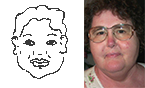
\includegraphics{111_2014_w_Kononova_face.png}
\end{center}

Программа, найдя на фотографии пациента похожее положение глаз, размер подбородка и др., выдаст нам результат о наличии или отсутствии травмы «Униженного». То же подходит и для других травм, только зависит от качества фотографий. Тело человека может содержать и несколько травм. Это потребует большего числа циклов обучения.

\subsubsection*{Вычисление диаграммы уровней мышления}

Согласно теории американского ученого К.~Грейвза, все живые системы в мире развиваются по спирали. По спирали также эволюционирует и мышление человека, приобретая четкие, характерные черты для каждого уровня мышления. Посредством онлайн теста можно построить для себя «диаграмму мышления» по типу jobEQ ASQ, ответив на некоторые вопросы:
\begin{center}
  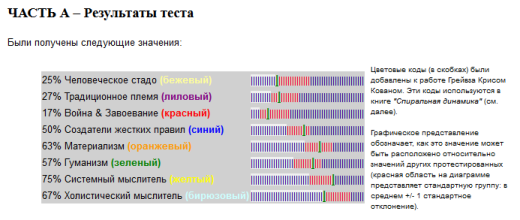
\includegraphics[width=0.8\textwidth]{111_2014_w_Kononova_results.png}
	Осуществляется такой тест на свободном движке, например, testMaker 3.3.
\end{center}

\subsubsection*{Лаборатория экспериментов PEBL}

PEBL "--- Psychology Experiment Building Language. Это простой язык программирования для создания различных экспериментов на основе шаблонов. С помощью его реализации PEBL 0.13 можно запускать написанные на PEBL скрипты. Хорошей демонстрацией возможностей языка является скрипт, генерирующий случайные числа для выявления проблем с памятью.

\subsubsection*{Обработка звука в Audacity}

Для выведения человека из состояния шока широко используются специальные звуковые дорожки, в которых правильно подобраны частоты сигнала. С помощью Audacity легко подготовить звуковые дорожки, например для следующих целей:
\begin{itemize}
 \item	Устранение шумов и изоляция лишних звуков из многослойной дорожки, чтобы научить клиента фокусировать внимание на отдельных фракциях звука (обучение концентрации внимания).
 \item	Волны человеческого голоса имеют разную громкость на разном уровне частот. Разделив дорожку собственного голоса клиента на части, можно продемонстрировать ему, буквально «на каких частотах» он разговаривает в обычной жизни. Это позволит задуматься, что именно стоит изменить в поведении и общении.
 \item	Для активизации правого полушария мозга человека психологи часто применяют вдохновляющую музыку. Компиляции из нескольких композиций удобно делаются в Audacity простыми инструментами монтажа.
\end{itemize}

Поскольку большинство программ используется психологами для прикладных целей, то можно сделать вывод: свободное ПО даже на сегодняшний день предлагает весьма солидный инструментарий и совершенно не уступает собственническому ПО.
	Тем не менее, вопрос о разработке централизованного ПО для психологов и коучей, которое собрало бы в себя новые течения, было бы высококачественным и при этом свободным, остается на сегодняшний день открытым.

\subsection*{Краткий словарь:}

Коучинг "--- персональный систематический психологический тренинг, в рамках которого тренер путем совместного с клиентом поиска решений, обеспечивает улучшение качества жизни, самообучение и личностный рост клиента. (перевод определения Association for Coaching)

Архетип "--- (от греч. arche "--- начало и typos "--- образ) Прообраз, первоначальный образ, идея. Был введен К.\,Г.~Юнгом, как древнешие общечеловеческие символы, лежащие в основе мифов, фольклора и культуры. В данном контексте под архетипами подразумеваются совокупности поведенческих моделей, характерных для того или иного человека.

«Дизайн человека» "--- одна из современных психологических теорий, в основе которой лежит предположение, что момент рождения человека четко определяет возможные ветви его развития. Знание о конкретном моменте позволяет выстроить довольно сложную «карту» эволюции личности. Интересна тем, что было предпринято множество попыток автоматизировать процесс построения Дизайна человека.

\end{document}
